\documentclass{article}
\usepackage[utf8]{inputenc}
% important for graphicx
\usepackage{graphicx}
\graphicspath{ {img/}{src/} }
\usepackage{float}
\usepackage{hyperref}
\usepackage{enumitem}
\usepackage{algorithm}
\usepackage{subcaption}
\usepackage[mathscr]{euscript}
\usepackage[detect-all]{siunitx}
\usepackage[noend]{algpseudocode}
% background color for definitions
\usepackage[most]{tcolorbox}
\tcbset{
    frame code={}
    center title,
    left=0pt,
    right=0pt,
    top=0pt,
    bottom=0pt,
    colback=blue!6!white,
    colframe=white,
    width=\dimexpr\textwidth\relax,
    enlarge left by=0mm,
    boxsep=10pt,
    arc=0pt,outer arc=0pt,
}


\newenvironment{changemargin}[2]{%
\begin{list}{}{%
\setlength{\topsep}{0pt}%
\setlength{\leftmargin}{#1}%
\setlength{\rightmargin}{#2}%
\setlength{\listparindent}{\parindent}%
\setlength{\itemindent}{\parindent}%
\setlength{\parsep}{\parskip}%
}%
\item[]}{\end{list}}

\begin{document}

\title{Image Processing II\\
 Watershed}
\author{Aadil Anil Kumar \\
Otmane Sabir
}
\date{29/2/2020}
\maketitle
\vspace{10mm}
\begin{center}
\section*{Introduction}
\large
The second homework assignment required us to implement the watershed transform while following certain guidelines which could be summarized to the following list: 
\vspace{7mm}
\begin{enumerate}
    \item Implement the watershed algorithm as described as pseudo code from the \hyperref[sec:hello]{\textcolor{blue}{textbook}} 4-connected and 8-connected neighborhood.
    \item Output a single CSV file for the transformed image in the same format and same definition and value domains as the input image 'f'.
    \item Do meaningful (motivated from a real-world perspective) watersheds for 3 other images.
\end{enumerate}
\end{center}
\newpage

\tableofcontents

\newpage

\section{Watershed Transform}
\vspace{2mm}
\begin{flushleft}
The watershed transform is a classical segmentation - separating different objects in an image - algorithm in the world of image processing; it initially derives from the the geological watershed which means the elevated terrain that separates neighboring drainage basins. The watershed transform segmentation follows the same logic: starting from defined markers, the watershed algorithm treats pixels values as a local topography (elevation). The algorithm floods basins from the markers until basins attributed to different markers meet on watershed lines. \textit{See Figure \ref{fig:watershed_visualization}}\newline
\vspace{2mm}
\end{flushleft}
\begin{figure}[ht]
    \centering
    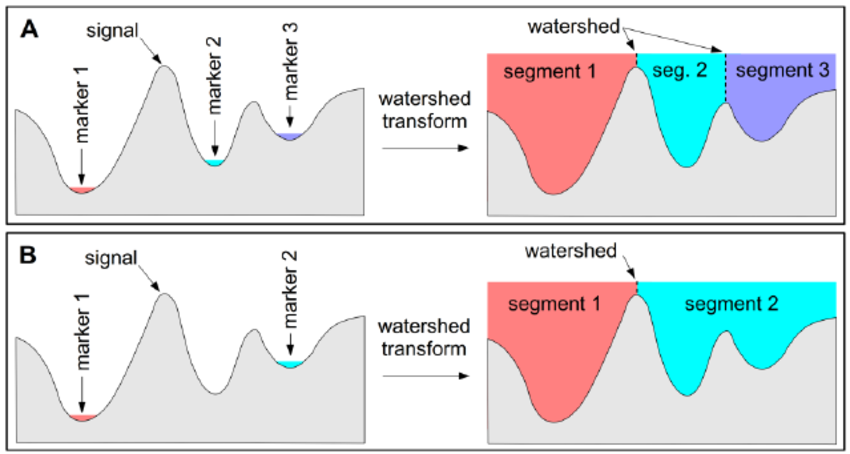
\includegraphics[width=8cm]{watershed.png}
    \caption{Watershed Visualization}
    \label{fig:watershed_visualization}
\end{figure}
\subsection{Formal Definition:}
\begin{flushleft}
\vspace{2mm }
\begin{tcolorbox}
\textsc{Definition:}\cite{parwshed} \newline\newline
Let $f \in C(D)$ have $minima$ $\{m_{k}\}_{k \in I}$, for some index set $I$. The catchment basin $CB(m_i)$ of a minimum $m_i$ is defined as the set of points $x \in D$ which are topographically closer to $m_i$ than to any other regional minimum $m_j$:
\begin{center}
\begin{equation*}
    CB(m_i) = \{x \in D | \forall j \textbackslash \in I\{i\} : f(m_i) + T_f(x, m_i) < f(m_j) + T_f(x, m_j)\}
\end{equation*}
\end{center}
\vspace{2mm}
The watershed of $f$ is the set of points which do not belong to any catchment
\begin{center}
\begin{equation*}
Wshed(f) = D \cap \left(\bigcup\limits_{i \in I} CB(m_i)\right)^c.
\end{equation*}
\end{center}
\vspace{4mm}
Let $W$ be some label, $W \notin I$. The watershed transform of $f$ is a mapping $\lambda : D \to I \cup \{W\}$, such that $\lambda(p) = i$ if $p \in CB(m_i)$, and $\lambda(p) = W$ if $p \in Wshed(f)$.
\newline\newline\newline
So the watershed transform of $f$ assigns labels to the points of $D$, such that $(i)$ different catchment basins are uniquely labelled, and $(ii)$ a special label $W$ is assigned to all points of the watershed of $f$.
\end{tcolorbox}
\end{flushleft}



\section{Algorithmic Definition}
\vspace{2mm}In our implementation, we're relying on the simulated immersion approach introduced by Vincent \& Soille \cite{soilletextbook}. \newline\newline
Metaphorically speaking, the algorithm pierces holes in every minimum, and the entire relief begins to be flooded with water. Starting from the minimum of lowest height, the water gradually fills up all catchment basins. Watersheds are built in the places where water from different basins unites. The process ends when the water reaches the maximum peak of the relief, and as a result, every catchment basin gets covered by the watershed lines which are easily distinguishable lines from the rest of the output.
\subsection{Formal Definition}
\begin{tcolorbox}
\textsc{Definition 2:} \cite{parwshed} \newline\newline
Let $f : D \to \N$ be a digital grey value image, with $h_{min}$ and $h_{max}$ the minimum and maximum value of $f$. Define a recursion with the grey level $h$ increasing from $h_{min}$ to $h_{max}$, in which the basins associated with the minima of f are successively expanded. Let $X_h$ denote the union of the set of basins computed at level $h$. A connected component to the threshold set $T_{h + 1}$ at level $h + 1$ can be either a new minimum, or an extension of a basin in $X_h$: in the latter case one computes the geodesic influence zone of $X_h$ within $T_{h+1}$, resulting in an update $X_{h+1}$. Let $MIN_h$ denote the union of all regional minima at altitude h.\newline\newline
Let us now define the following recursion: \newline
\[
\begin{cases}
    X_{h_{min}} = & \{p \in D | f(p) = T_{h_{min}}\}\\
    X_{h+1} = & MIN_{h+1} \cup IZ_{T_{h+1}}\left(X_h\right), h \in [h_{min}, h_{max})
\end{cases}
\]
\newline\newline
The watershed $Wshed(f)$ of $f$ is the complement of $X_{h_{max}}$ in $D$ : 
\begin{center}
    $Wshed(f) = D \textbackslash X_{h{max}}$
\end{center}
\end{tcolorbox}
\vspace{2mm}
\begin{flushleft}
Let's use Figure \ref{fig:example_1} from \cite{parwshed} as an example of the algorithm defined above. Assuming that A and B are basin labels and that W is the watershed pixels. Then the algorithm will proceed as shown in the figure (a) is the original image and the (b-e) are steps following the algorithm definition above.
\end{flushleft}

\begin{figure}[H]
    \centering
    \includegraphics[width=\linewidth]{example1.png}
    \caption{Immersion algorithm on the 4-connected grid}
    \label{fig:example_1}
\end{figure}

\subsection{Implementation}
As we previously discussed, we attempted to implement the immersion approach. The pseudo code \href{alg:immersion_alg} below was provided by Soille \cite{soilletextbook}.
\newline

\subsubsection{Pixel Mapping}
\subsubsection{Neighbouring Pixels}
\subsubsection{Queue Data Structure}

\newpage

\vspace*{-3cm}

\begin{algorithm}[H]
\caption{Watershed using flooding simulations}\label{euclid}
\begin{algorithmic}[1]
\label{alg:immersion_alg}
\Procedure{watershed}{}
\State $\textit{mask} \gets \text{-2  ;  }  \textit{initial value of a threshold level}$
\State $\textit{wshed} \gets \text{0  ;  }  \textit{value of pixels belonging to watersheds}$
\State $\textit{inqueue} \gets \text{-3  ;  } \textit{value assigned to pixels put into the queue}$
\State $\textit{init} \gets \text{-1  ;  } \textit{initial value of f0)}$
\newline
\BState \emph{Input : $f_i$}, \text{grey tone image (non negative integers)}:
\BState \emph{Output : $f_0$}, \text{image of labelled catchment basins}:
\newline
\Procedure{Initialisations}{}
\BState \text{Value} \emph{$f_i$} \text{is assigned to each pixel of $f_0$}:
\BState \emph{current\_label} $\gets$ \text{0}:
\BState \emph{flag: } \text{Boolean variable}:
\BState \emph{$N(p)$} \text{is the set of neighbours of P}:
\EndProcedure
\newline
\BState \textbf{Sort} the pixels of $f_i$ in the increasing order of their grey values. \newline
\For{$h \gets h_{min}$ \textbf{to} $h_{max}$}
\Comment{geodesic SKIZ of level h - 1 inside level h}
    \For{pixel p}
    \Comment{such that $f_{i}(p) = h$}
        \BState $f_{0}(p) \gets$ \text{mask}
        \If{ $\exists$ p' $\in$ N(p) | $f_{0}(p') > 0$ \textbf{OR} $f_{0}(p')$ = wshed}
            \BState \emph{$f_{0}(p) \gets$ inqueue}
            \Comment{fifo.add(p)};
        \EndIf
    \EndFor
\EndFor
\While{fifo.empty() = false}
    \BState p $\gets$ fifo.retrieve();
    \For{pixel p' $\in N(p)$}
        \If{$f_{0}(p') > 0$}
        \Comment{i.e., p' belongs to an already labelled basin}
            \If{$f_{0}(p) = $ inqueue \textbf{OR} ($f_{0}(p) = $ wshed \textbf{\&} flag = true)}
                \State $f_{0}(p)$ \gets $f_{0}(p')$
            \ElsIf{$f_{0}(p) >$  0 \textbf{AND} $f_{0}(p) \neq f_{0}(p')$}
                \State $f_{0}(p) \gets wshed$
                \Comment{flag $\gets$ false}
            \EndIf
        \EndIf
        \ElsIf{$f_{0}(p') = $ wshed}
            \If{$f_{0}(p) = $inqueue}
                \State $f_{0}(p) \gets$ wshed;
                \State flag $\gets$ true;
            \EndIf
        \ElsIf{$f_{0}(p')$ = ,ask}
            \State $f_{0}(p) \gets$ inqueue;
            \State $f_{0}(p') \gets$ mask;
        \EndIf
    \EndFor
    \For{pixel p} 
    \Comment{such that $f_{i}(p)$ = mask}
        \If{$f_{0}(p)$ = mask}
        \Comment{check for new minima}
            \State current\_label $\gets$ current\_label + 1;
            \State fifo.add(p);
            \State $f_{0}(p) \gets $ current\_label;
            \While{fifo.empty() = false}
                \State $p' \gets$ fifo.retrieve();
                \For{p" $\in N(p')$}
                    \If{$f_{0}(p'')$ = mask}
                        \State fifo.add(p'');
                        \State $f_{0}(p'') \gets$ current\_label;
                    \EndIf
                \EndFor
            \EndWhile
        \EndIf
    \EndFor    
\EndWhile
\EndProcedure
\end{algorithmic}
\end{algorithm}

\section{Experiments & Results}


\section{Comparison}
The breadth-first implementation that we're discussing uses a FIFO (First in First Out) queue to find the level of pixels of constant grey value as we have seen, c.f Algorithm \ref{alg:immersion_alg}. For each of these thresholds a pixel is stored in the empty queue, followed by the 'flooding' which runs until the queue is empty. 
\subsection{Time Complexity}

\begin{flushleft}
We ran some tests on the algorithm which was presented in order to visualize the time complexity of this algorithm. 
We can clearly see that the time complexity is linear in the number of pixels in the image; however, according \cite{timecomplexity} the theoretical time complexity would change from linear to quadratic due to the repeated processing of the watershed pixels.

\end{flushleft}

\begin{figure}[ht]
\centering
\begin{subfigure}{.5\textwidth}
  \centering
  \includegraphics[width=\linewidth]{tests/performane_8.png}
  \caption{8 - Neighbours}
  \label{fig:sub1}
\end{subfigure}%
\begin{subfigure}{.5\textwidth}
  \centering
  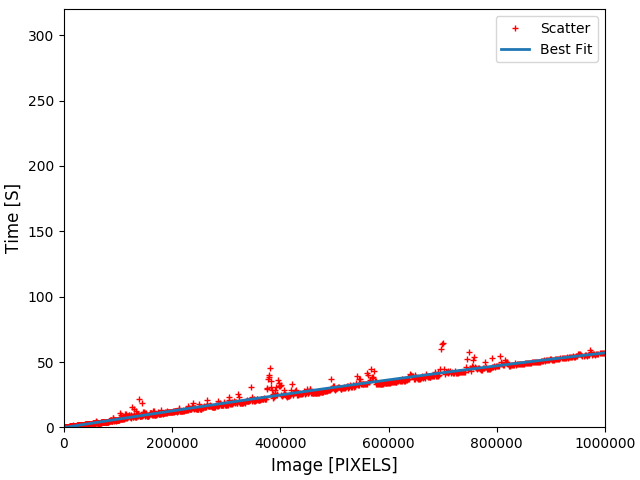
\includegraphics[width=\linewidth]{tests/performance_4.png}
  \caption{4 Neighbours}
  \label{fig:sub2}
\end{subfigure}
\caption{Scatter Plot  \& Best Fit curve of results}
\label{fig:general_test}
\end{figure}

\begin{figure}[ht]
    \centering
    \includegraphics[width=\linewidth]{neighbor-chartbar.png}
    \caption{Different neighbors bar chart.}
    \label{fig:neighbor-chartbar}
\end{figure}

\subsection{N-Neighbors Influence}
\begin{flushleft}
After the previous tests, we noticed how the number of neighbors scanned impacts the time the algorithm; therefore, we decided to run different test with various neighbor sizes (2, 4, 8, 16) and visualized the differences as seen in  Figure~\ref{fig:neighbor-test}. We ran a test on random graphs of size [n , n] with n ranging from \numrange[range-phrase = -- = --]{1}{500}. We also ran a test, c.f \ref{fig:neighbor-chartbar} using 2, 4, 6, 8, 16, 32, and 64 to be able to determine how exactly the amount of neighbors influences the overall run time of the algorithm on a 512*512 image.

This helps us explain how the algorithm heavily depends on its neighbors and why, as previously mentioned, the time complexity can vary from linear to quadratic. We almost always see a doubling the overall time until we reach 64 neighbors and notice a much more significant jump.
\end{flushleft}

\begin{figure}[H]
  \begin{subfigure}{6cm}
    \centering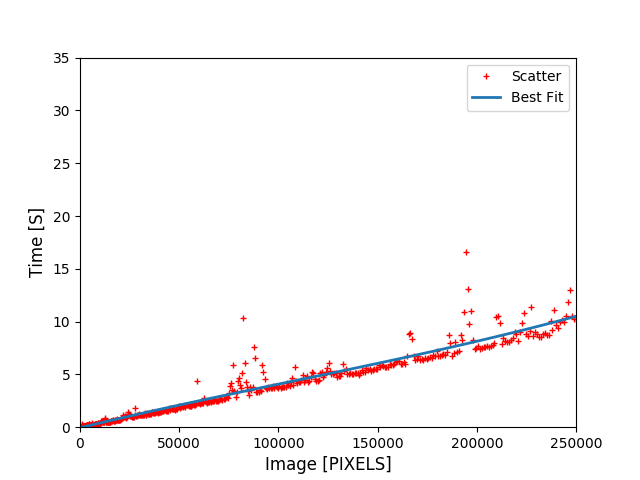
\includegraphics[width=6cm]{tests/test_ws_2.png}
    \caption{2 - Neighbors}
  \end{subfigure}
  \begin{subfigure}{6cm}
    \centering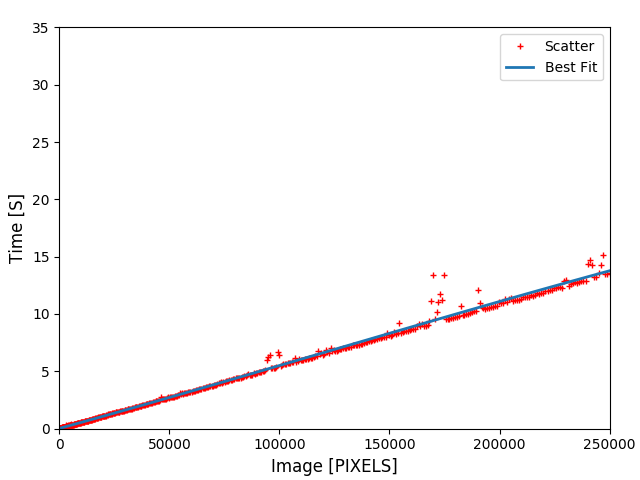
\includegraphics[width=5.5cm]{tests/test_ws_4.png}
    \caption{4 - Neighbors}
  \end{subfigure}
 
  \begin{subfigure}{6cm}
    \centering\includegraphics[width=6cm]{tests/test_ws_8.png}
    \caption{8 - Neighbors}
  \end{subfigure}
  \begin{subfigure}{6cm}
    \centering\includegraphics[width=5.5cm]{tests/test_ws_16.png}
    \caption{16 - Neighbors}
  \end{subfigure}
  \caption{Scatter Plot \& Best Fit curve for different neighbors}
  \label{fig:neighbor-test}
\end{figure}



\subsection{The queue disadvantages}
\begin{flushleft}
One of the main advantages of this algorithm is how it utilizes the queue to reduce time complexity and keeps all our operations feasible in linear time but this also comes at a cost. When running our initial test, we tried running multiple processes at the same time in for optimal performance; however, we ran into many issues because of the nature of the algorithm. The required size of the queue is not known in advance, and memory is addressed in a very unstructured and "blind" manner, causing performance degradation on
virtual memory and especially on parallel computing, since it requires a lot of synchronization and tends to leave with many imprecise results. In the figures below you can clearly see the difference when running the processes concurrently vs. running them in normal linear manner.
\end{flushleft}

\begin{figure}[ht]
\centering
\begin{subfigure}{.5\textwidth}
  \centering
  \includegraphics[width=\linewidth]{tests/concurent.png}
  \caption{Concurrent Testing}
  \label{fig:sub1}
\end{subfigure}%
\begin{subfigure}{.5\textwidth}
  \centering
  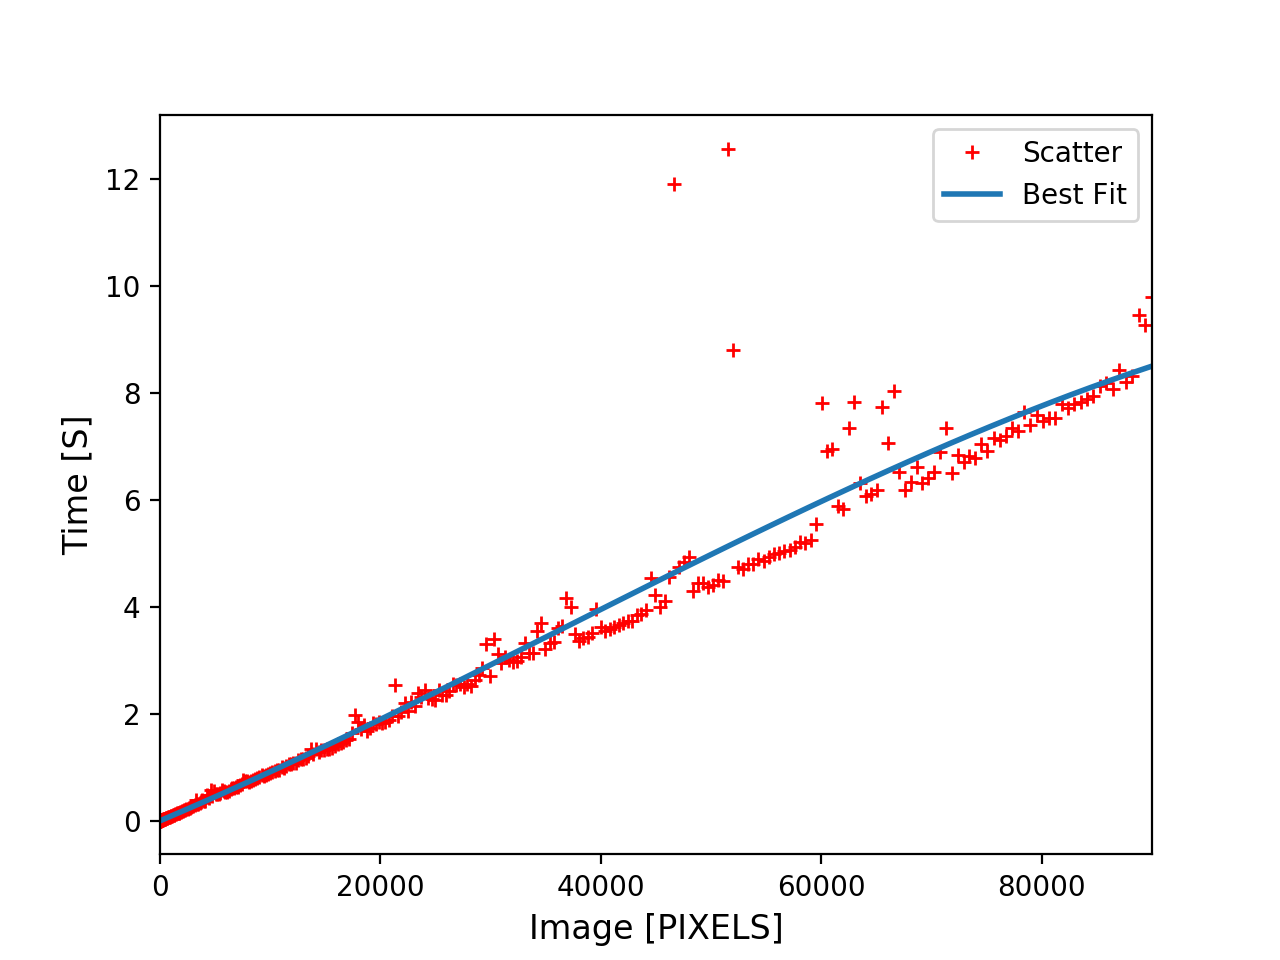
\includegraphics[width=\linewidth]{tests/consecutive.png}
  \caption{Consecutive Testing}
  \label{fig:sub2}
\end{subfigure}
\caption{Scatter Plot  \& Best Fit Cruves for Consecutive and Concurrent testing. }
\label{fig:concurrency_test}
\end{figure}


\section{Task Distribution}
\begin{flushleft}
TEXT GOES HERE
\end{flushleft}

\newpage

\begin{thebibliography}{9}
\label{sec:hello}



\bibitem{parwshed}
Jos B.T.M. Roerdink and Arnold Meijster : \newline
Institute for Mathematics and Computing Science, 
\\\texttt{http://www.cs.rug.nl/roe/publications/parwshed.pdf}


\bibitem{soilletextbook} 
Soille, P. (2010). Morphological image analysis: principles and applications. 
\textif{Berlin: Springer. Samarin}. 

\end{thebibliography}

\end{document}
